\documentclass[lualatex,a4paper]{bxjsarticle}
\usepackage{luatexja-fontspec}
\usepackage[luatex]{graphicx,color}
\usepackage{amsmath}
\usepackage{amsthm}

\topmargin=-2.0cm
\textheight=25.0cm
\textwidth=17.0cm
\oddsidemargin=-1.0cm
\evensidemargin=-1.0cm
\renewcommand{\baselinestretch}{0.95}

\title{\bf テスト}
\author{B4 お茶 花子}

\begin{document}
\twocolumn{
	\maketitle
}

\section{テスト}

\begin{enumerate}
	\item い
	\item ろ
	\item は
\end{enumerate}

引用\cite{test-bib}

\begin{figure}
	\begin{center}
		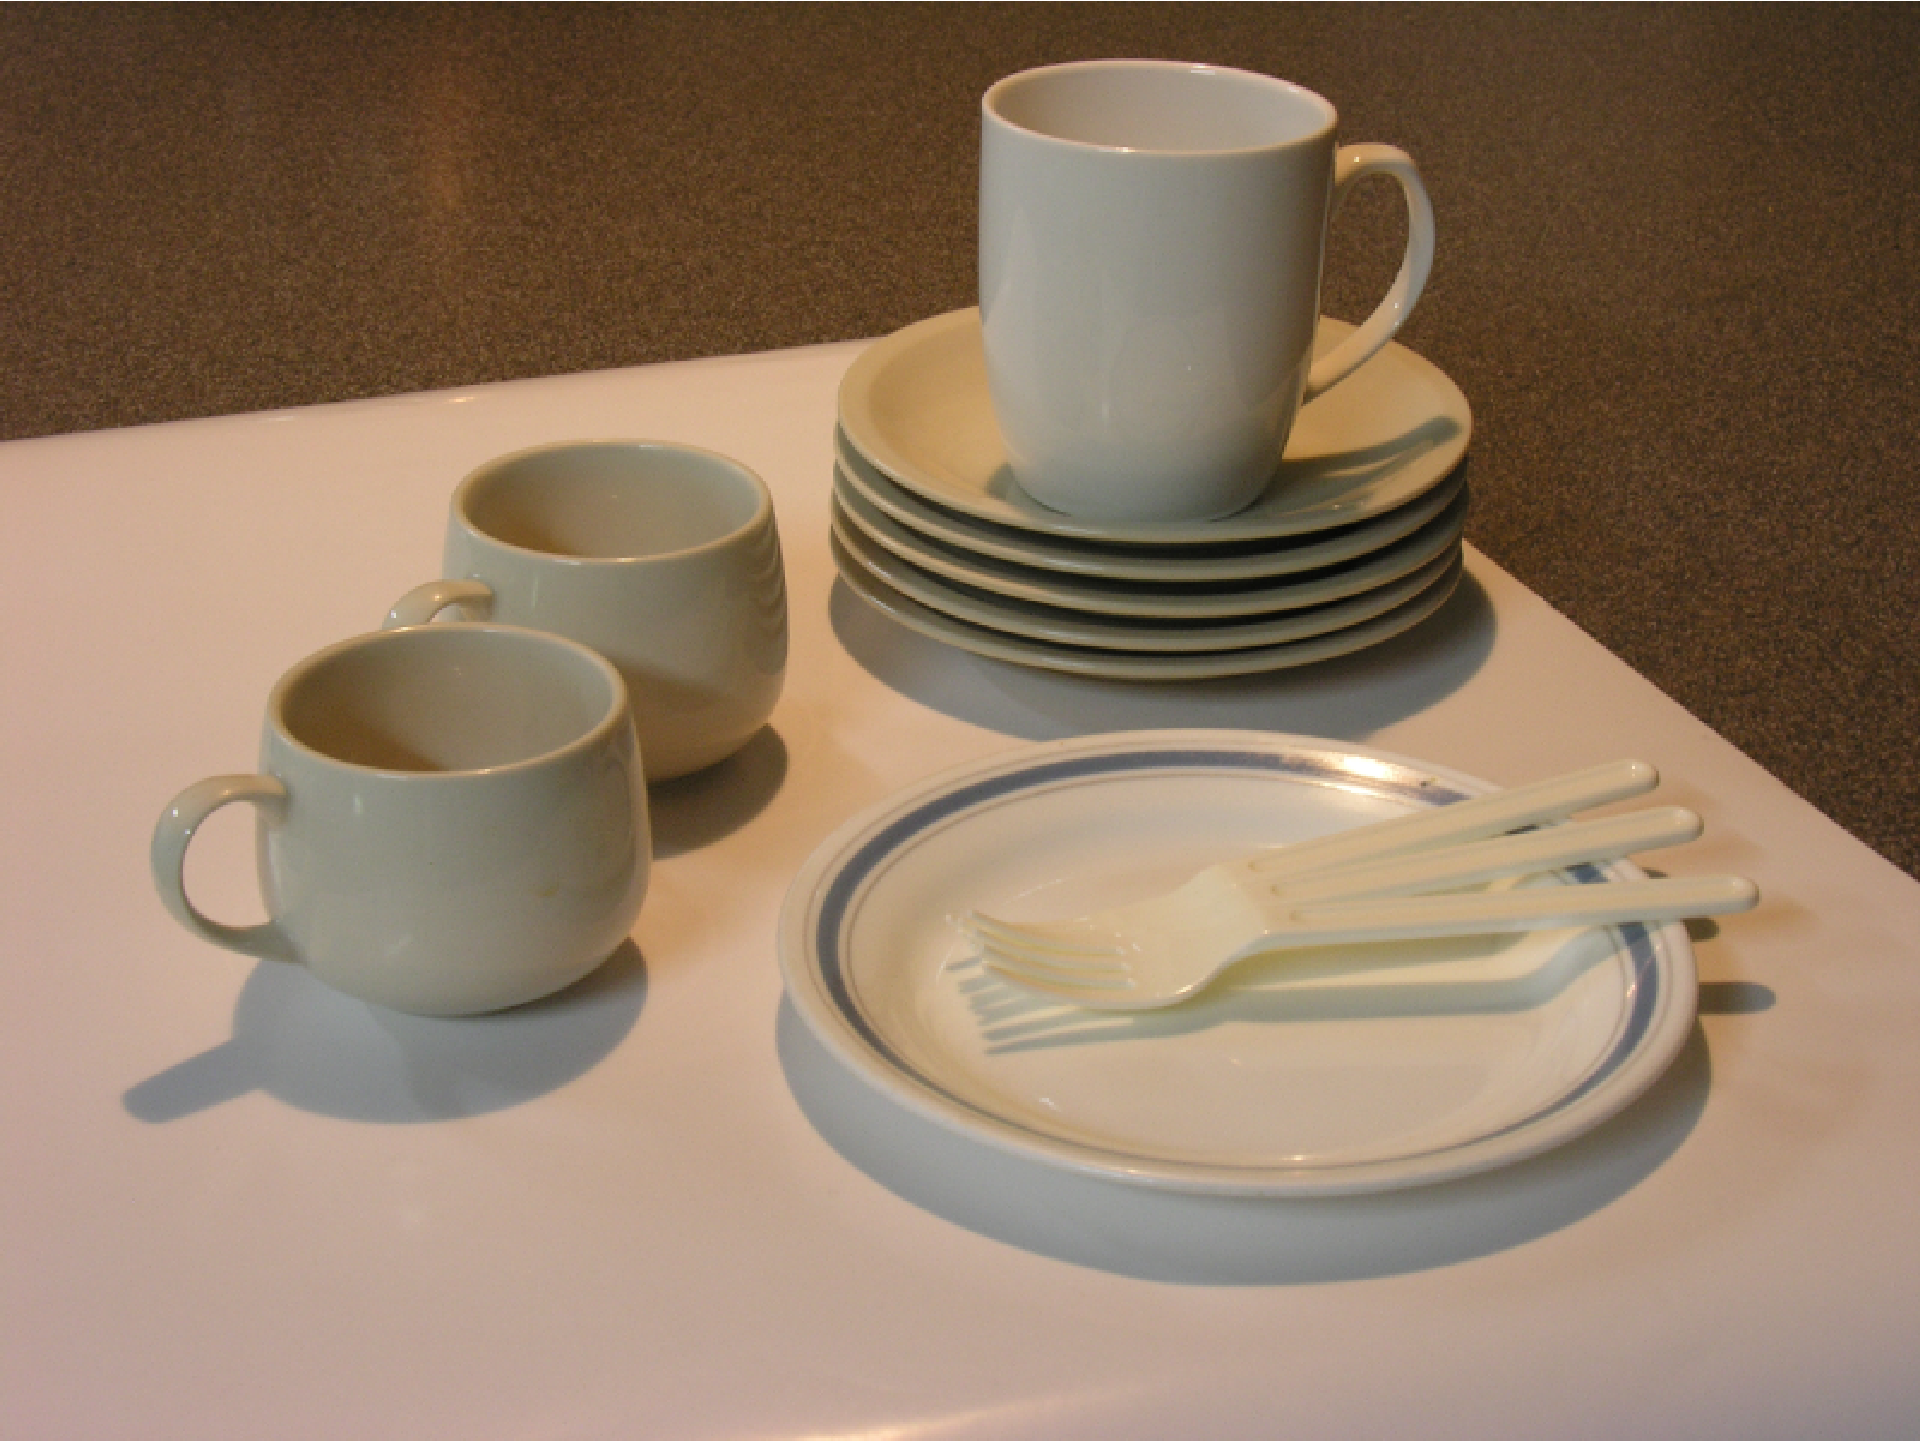
\includegraphics[width=\linewidth]{cups.png}
	\end{center}
	\caption{画像}
	\label{fig:cups}
\end{figure}

\bibliographystyle{junsrt}
%\nocite{*}
\small
\bibliography{references} %参考文献データの入ったファイル名をここに書
%きます.

\end{document}
